%
% File acl2018.tex
%
%% Based on the style files for ACL-2017, with some changes, which were, in turn,
%% Based on the style files for ACL-2015, with some improvements
%%  taken from the NAACL-2016 style
%% Based on the style files for ACL-2014, which were, in turn,
%% based on ACL-2013, ACL-2012, ACL-2011, ACL-2010, ACL-IJCNLP-2009,
%% EACL-2009, IJCNLP-2008...
%% Based on the style files for EACL 2006 by 
%%e.agirre@ehu.es or Sergi.Balari@uab.es
%% and that of ACL 08 by Joakim Nivre and Noah Smith

\documentclass[11pt,a4paper]{article}
\usepackage[hyperref]{acl2018}
\usepackage{times}
\usepackage{latexsym}

\usepackage{csquotes}
\usepackage{graphicx}

\usepackage{url}

\aclfinalcopy % Uncomment this line for the final submission
%\def\aclpaperid{***} %  Enter the acl Paper ID here

%\setlength\titlebox{5cm}
% You can expand the titlebox if you need extra space
% to show all the authors. Please do not make the titlebox
% smaller than 5cm (the original size); we will check this
% in the camera-ready version and ask you to change it back.

\newcommand\BibTeX{B{\sc ib}\TeX}

\title{Class project: Complex Word Identification}

\author{Pierre Finnimore}

\begin{document}
\maketitle
%\begin{abstract}
%
%\end{abstract}

\section{Introduction}

The task is as follows: given a target word (or set of words) within a sentence, identify if the target is \enquote{complex}. The data given for this task is a set of labelled sentences with targets. The labels were derived from a survey of both Native and Non-native speakers of two languages: English and Spanish.

We are interested in identifying word complexity for several reasons. Automatic extraction of complex terms could help with automated tutoring systems, Natural Language Generation, writing editing software, studies into second-language acquisition, political speech analysis, Machine Translation, as well as linguistic or psychological studies into the what people find complex. 

\section{Baseline system description}

The baseline system we developed was more advanced than the initial baseline provided. Both languages used an identical model and set of features. We focused on features that could be extracted using only the target word; no context words were considered.

Our initial hypotheses to try for the baseline were as follows:
\begin{enumerate}
\item Letter rarity - this feature was chosen because words with rarer letters might be harder to understand. This feature could be seen as a vague approximation of word rarity, which would otherwise require more data to learn.
\item Max consecutive consonants, max consecutive vowels - the idea behind this was that dense combinations of letters might be difficult to parse. For example "queueing" or "rhythms". These words deviate from the more straightforward consonant-vowel-consonant-vowel pattern.
\item Uniquely English vowel/consonant diagraphs/consonant blends - this was chosen because a non-English speaker might find these tricky.
\item POS tags - because some POS are part of closed sets, and so potentially easier to understand. In addition, certain rarer tags might be harder to comprehend, especially in languages where the overall form of the word is changed, depending on its POS.
\item Number of synonyms - The idea was that ambiguous words might be more confusing. Conversely, perhaps ambiguous words are actually less likely to be regarded as complex, since it is more likely that the person knows at least one of the meanings.
\end{enumerate}

While individually, these features allowed the system to predict with greater-than-random accuracy, most of them did not improve over the baseline. Some of the features we tried, such as Spanish prefixes, reduced the testing accuracy if they were added. This may just be noise in the data, or it may be that learning is made more difficult if irrelevant features are added. This provided some motivation to try different learning models.

We identified that POS tags were computationally costly, while not providing performance improvements, and so removed them. Our final Baseline System used the following features: No. of words and characters in the target, \enquote{Rarity} score based on the target's letters, Maximum no. of consecutive vowels and consonants, No. of synonyms, Common English and Spanish Prefixes, Infixes and Suffixes, and Common Latin and Greek prefixes.

\begin{table}[h]
\begin{center}
\begin{tabular}{|c|c|c|}
\hline
\textbf{Language} & \textbf{LR} & \textbf{RFC} \\
\hline
English & 0.73 & 0.81 \\ \hline
Spanish & 0.74 & 0.75 \\ \hline
\end{tabular}
\caption{Macro-F1 Score for baseline system, with logistic regression (LR) and random forest classifier (RFC)}
\label{tab:baseline}
\end{center}
\end{table}

\begin{table}[h]
\begin{center}
\begin{tabular}{|c|c|c|}
\hline
\textbf{Language} & \textbf{LR} & \textbf{RFC} \\
\hline
English & 0.77 & 0.82 \\ \hline
Spanish & 0.77 & 0.74 \\ \hline
\end{tabular}
\caption{Macro-F1 Score for advanced system, with logistic regression (LR) and random forest classifier (RFC)}
\label{tab:advanced}
\end{center}
\end{table}

As seen in Table \ref{tab:baseline}, it achieved performance of 0.73 on English and 0.74 on Spanish with a logistic regression approach on the development data. For the advanced system, seen in Table \ref{tab:advanced}, we implemented Random Forest Classifiers, and when we tried this on the baseline system, achieved performance of 0.81 and 0.75 for English and Spanish respectively.

\section{Improved system motivation and description}

One of the features added to the advanced system was extracted from a list of \enquote{1000 simple English words} on Wikipedia. We used these to extract sub-word features of two or three letters. The idea was that these words contained certain patterns that people regard as simple. Each sub-word feature was weighted by how often it occurred in the text. Interestingly, introducing these features improved the Spanish F-score, but not the English F-score. This may be because those combinations also happened to correlate with easy or difficult morphological features in Spanish, or it may be that the participants of the original study found that combinations that they recognised from English were easier or more difficult to identify in Spanish.

The single largest improvement to the model was obtained by using a Random Forest Classifier rather than a Logistic Regression classifier. To understand why it is effective, it is easiest to start with thinking about a simple decision tree. A decision tree is a sequence of decisions, based on the features supplied, which partition the result space. If we were making our own decision tree for this task, we might think something like \enquote{Is the word longer than 10 letters? If yes, it is complex. If no, does the word end with \enquote{ough}? If yes, it is complex. Otherwise, it isn't.}. This set of rules, which partition the classes effectively, can be learned by the computer. 

However, there are issues with simple decision trees. Since we do not know ahead of time what the optimal partitions are, we take an approach where we see at each decision point how to partition the features such that it splits the data. But this will only guarantee locally good splits: there may be a different split that leads to globally better partitions. In addition, they are likely to overfit as the partitions get small. This is where Random Forests are useful. They can take a set of simple decision trees, each trained on a different subset of the features, and make a decision based on all of those smaller decisions. In a way, we could think about each simple decision tree extracting some feature or cluster of features, like the \enquote{length + ough-suffix}, and the Random Forest learns how to make decisions based on these more sophisticated, abstracted features. 

This is somewhat analagous to the hidden layers of a neural network, where first we reduce the dimensionality of our data to features, then we reduce the dimensionality of our features to a set of abstracted feature-combinations, and only \emph{then} make our decision.

 There are several reasons that we might think that a Random Forest Classifier would be a promising candidate for a task such as this. First, it produces the aforementioned abstracted feature-combinations. Additionally, it enables analysis of feature importance, making further directions for development easier to identify. Finally, there is precedent for use of this approach in NLP. For example, Treeratpituk and Giles \citep{treeratpituk2009disambiguating}
used Random Forests for the task of disambiguating author names. They found that Random Forests outperformed Naive Bayes, Logistic Regression and SVMs, while having shorter training times than SVMs. More specifically, Gonzalez-Dios et al. \cite{gonzalez2014simple} found that a Random Forest approach was comparable to SVMs for the task of Complexity analysis of the Basque language.



When we used the Random Forest Classifier, we took a look at the most important features for each model, seen in Tables \ref{tab:EngFeats} and \ref{tab:SpFeats}. As expected, \enquote{Number of characters in target} and \enquote{Number of tokens in target} were the number 1 and 2 spots for importance for both languages. Interestingly, the \enquote{Rarity score}, which we developed as a basic measure of the use of rare letters in the word was the 3rd most important feature for English and 4th most important feature for Spanish. 

\begin{table}[h]
\begin{center}
\begin{tabular}{|c|l|c|}
\hline
\textbf{Rank} & \textbf{Feature} & \textbf{Importance} \\
\hline
1. & Number of characters & (0.106) \\ \hline
2. & Synonym count & (0.0397) \\ \hline
3. & Number of tokens & (0.0378) \\ \hline
4. & Rarity score & (0.0358) \\ \hline
5. & Max cons. consonants & (0.0142) \\ \hline
6. & Suffix: ed & (0.00915) \\ \hline
7. & Bi: ed & (0.00894) \\ \hline
8. & Infix: r & (0.00851) \\ \hline
9. & Max cons. vowels & (0.00737) \\ \hline
10. & Bi: ti & (0.00669) \\ \hline
\end{tabular}
\caption{Top 10 English Features}
\label{tab:EngFeats}
\end{center}
\end{table}

\begin{table}[h]
\begin{center}
\begin{tabular}{|c|l|c|}
\hline
\textbf{Rank} & \textbf{Feature} & \textbf{Importance} \\
\hline
1. & Number of tokens & (0.0894) \\ \hline
2. & Number of characters & (0.076) \\ \hline
3. & Rarity score & (0.0441) \\ \hline
4. & Max cons. consonants & (0.0246) \\ \hline
5. & Bi: de & (0.0115) \\ \hline
6. & Synonym count & (0.0109) \\ \hline
7. & Infix: r & (0.0099) \\ \hline
8. & Max cons. vowels & (0.00914) \\ \hline
9. & Suffix: a & (0.00805) \\ \hline
10. & Suffix: s & (0.00725) \\ \hline
\end{tabular}
\caption{Top 10 Spanish Features}
\label{tab:SpFeats}
\end{center}
\end{table}

It is important to note that we may be getting the wrong impression from these importance scores, since each feature is measured independently. While there is only one \enquote{Number of synonyms} feature, there are 312 \enquote{Two-letter infix} features and \textit{1297} \enquote{Three-letter infix} features. While any given infix feature may be less significant than these more comprehensive, overall features, the sum total of their effect may be greater.

We ran several experimenets with different numbers of trees for the Random Forest Classifier, and found that 20 produced the best results. We also found that a basic logistic regression was more effective for Spanish, so we separated the model approaches for the two languages.

\section{Experiments on development set}

\begin{table}[h]
\begin{center}
\begin{tabular}{|c|c|c|c|}
\hline
\textbf{Data} & \textbf{System} & \textbf{Language} & \textbf{Score} \\
\hline \hline
Dev. & Baseline & English & 0.81 \\ \hline
Test & Baseline & English & \textbf{0.82} \\ \hline \hline
Dev. & Advanced & English & 0.82 \\ \hline
Test & Advanced & English & \textbf{0.82} \\ \hline \hline
Dev. & Baseline & Spanish & 0.73 \\ \hline
Test & Baseline & Spanish & \textbf{0.75} \\ \hline \hline
Dev. & Advanced & Spanish & 0.77 \\ \hline
Test & Advanced & Spanish & 0.74 \\ \hline
\end{tabular}
\caption{Macro-F1 Score on Development and Test data, for different systems and languages. Best result for each language on the test data is highlighted. For both the baseline system, RFC was used, since it provided the best results in later experiments}
\label{tab:testdev}
\end{center}
\end{table}

Interestingly, while the advanced system did particularly well on the development data, it did not perform so well on the test data, being outperformed by the baseline system. This suggests that the fact that Logistic Regression seemed effective for the advanced system may have been a case of overfitting to the development data. This highlights the importance of keeping the test set separate.  The baseline system also improved on its performance for the English language, becoming on-par with the advanced system. This potentially suggests that the additional features added to the advanced system did not provide significant benefits. So by Occam's razor, the simpler, baseline system, should be preferred.

Some of the ideas that we tried worked, but not in the expected way. For example, the case mentioned in the previous section, where adding subword features from 1000 simple English words improved the Spanish score. However, it appears that there is some linguistic research to suggest why this may be the case: Morphology may be particularly important to Spanish learners.

Some of the targets that the advanced system predicted correctly, while the baseline system predicted incorrectly: \emph{flooding, hospitals, clinics, eroding, internationally brokered peace plan, amateur, ducked, pilgrimage, Guerreros, Calabria, Atenas, cercanías, datación, procedencia, esculturas, asociación, Praga, estudio}. Qualitatively, compared with the words that both systems correctly predicted, these words appear to have more unusual letter combinations, which may explain why the more robust sub-word features in the advanced system were effective.

\section{Learning curves}

\begin{figure}[h]
\begin{minipage}[b]{1.0\linewidth}
  \centering
  \centerline{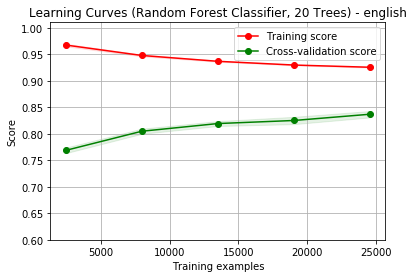
\includegraphics[width=7.5cm]{images/RFCEng}}
\end{minipage}
\begin{minipage}[b]{1.0\linewidth}
  \centering
  \centerline{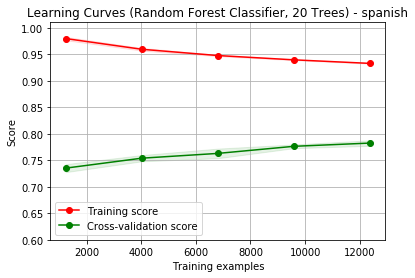
\includegraphics[width=7.5cm]{images/RFCSp}}
\end{minipage}
\caption{5-fold cross validation performance on English and Spanish training data for a Random Forest Classifier with 20 Trees}
\label{fig:RFC}
\end{figure}

In general, the systems seen in Figs. \ref{fig:RFC} and \ref{fig:Log} indicate that the Spanish data is more difficult to learn from, with a lower starting point and shallower improvements as more data was added. This may be a peculiarity of the dataset that we had, or representative of the nature of the language itself.

\begin{figure}[h]
\begin{minipage}[b]{1.0\linewidth}
  \centering
  \centerline{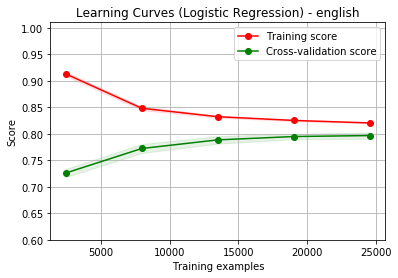
\includegraphics[width=7.5cm]{images/LogEng}}
\end{minipage}
%\begin{minipage}[b]{1.0\linewidth}
%  \centering
%  \centerline{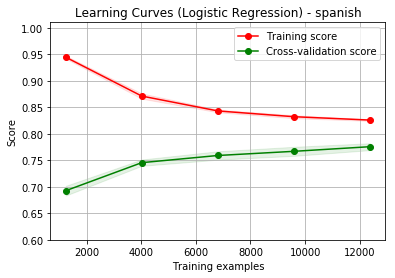
\includegraphics[width=7.5cm]{images/LogSp}}
%\end{minipage}
\caption{5-fold cross validation performance on English training data for a Logistic Regression}
\label{fig:Log}
\end{figure}

The curves for the logistic regression approach in Fig. \ref{fig:Log} are converging to a greater extent than those of the Random Forest Classifier seen in Fig. \ref{fig:RFC}. This suggests that adding more training data would do little for the logistic regression approach, whereas there are still potential gains to be had for the Random Forest Classifier, if more data were available.

With little data available, the Random Forest Classifier still outperforms the Logistic Regression approach. In general, the approaches that we would expect to take the most data would be those based on neural networks, since back-propagation requires very small steps along the gradient. However, since we did not implement these techniques, we did not encounter this difficulty.



\section{Examples of failed predictions}

Some examples of situations where \emph{both} the advanced system and the baseline system failed were: \emph{internationally, calm, amateur video, wounds, treatment, Coordination, Committees, has been awakened, Mariottini, investigación, identidad, encontradas, auriga, Regio, exponen, griegas, Riace, Bronces}. At least for the English words, many of the situations where both systems predicted incorrectly were very common words. Potentially scraping wikipedia or other large data-sources for word frequencies (or even sub-word frequencies) would be effective. For the Spanish words, words like \enquote{investigación} are extremely similar to English words, yet predicted incorrectly. Perhaps a feature that captured longer suffixes like \enquote{ción} and \enquote{tion} would be helpful.

\section{Conclusions}

Our main approach to this task was to find some data, then try to extract as much as we could from that data. We primarily focussed on subword features, as these effectively reduce sparsity. These subword features proved to be effective at this task, suggesting that at least one component of perceived complexity is simply the structure of the word's constituent letters. On a more \enquote{meta} level, our system improved as we introduced more data to the features.

% include your own bib file like this:
%\bibliographystyle{acl}
%\bibliography{acl2018}

\bibliography{mybib}
\bibliographystyle{acl_natbib}

\end{document}
